\documentclass[11pt,a4paper]{article}
\usepackage[utf8]{inputenc}
\usepackage[T1]{fontenc}
\usepackage{amsmath,amssymb}
\usepackage{graphicx}
\usepackage[margin=2.7cm]{geometry}
\usepackage{booktabs}
\usepackage[colorlinks=true,linkcolor=blue,citecolor=blue,urlcolor=blue]{hyperref}
\usepackage{xcolor}

\newcommand{\figplaceholder}[2]{%
  \begin{center}\fbox{\parbox{0.86\textwidth}{\centering\vspace{2.2cm}%
  \textbf{Figure #1 (placeholder)}\\[2pt]\small #2\vspace{2.2cm}}}\end{center}}

\title{Counting laws of links in Poisson-sprinkled causal sets:\\
IR-cutoff valency, FRW transients, and three-sector accounting}
\author{Patricio Fernando Bustos Cabrera}
\date{Draft --- July 2026}

\begin{document}
\maketitle

\begin{abstract}
In a causal set faithfully embedded in a continuum spacetime, the valency of an
element---its number of links, i.e.\ covering relations---is infinite in the
absence of a cutoff. We measure and derive the growth laws of past valency
under an explicit IR cutoff for three geometries. (i)~In 1+1 Minkowski the
per-element past valency grows logarithmically, $v = 2\ln(T\sqrt{\rho})$; the
measured slope is $2.01 \pm 0.12$ and is insensitive to the sprinkling size
(tested over an eightfold range in $N$), confirming that valency is a local
quantity controlled by chain depth rather than by the global element count.
(ii)~In 3+1 Minkowski the valency obeys an area law,
$v = \pi\sqrt{6}\,\sqrt{\rho}\,T^{2}$, with measured exponent
$2.089 \pm 0.025$ and amplitude agreeing with the parameter-free prediction
$\kappa_{4}=\pi\sqrt{6}$ at the 5\% level. (iii)~In a matter-dominated FRW
interval the area law survives with a derived blocking amplitude
$\mathfrak{F} = 30\int_{0}^{1} x(1-x)^{8}/\sqrt{\langle a^{4}\rangle}\,dx
= 0.4991$, against a measured $0.4990$---four-figure agreement---preceded by
an explicit $1/\eta$ transient that we fit and subtract. We further show that
the link fraction $\varepsilon = N_{\mathrm{links}}/N_{\mathrm{past}}$ follows
$\varepsilon = 3\sqrt{6}/(\sqrt{\rho}\,R^{2})$ and cleanly separates
manifoldlike sprinklings ($\varepsilon \approx 0.21$ at our reference scale)
from transitively-closed random orders ($\varepsilon \approx 0.017$). The
pipeline is anchored to the literature by reproducing the interval-abundance
baseline $\langle N_{0}\rangle$ of Glaser \& Surya in a 4D diamond to
$0.07\sigma$. We close with a chain/antichain partition identity for weakly
disformal metrics---a counting consistency statement, not a dynamical
result---and the pre-registered experiment that will test whether its
exponents arise from biased growth dynamics. All results are
deterministic-seed reproducible; code and pre-registrations are public.
\end{abstract}

\section{Introduction}

A causal set is a locally finite partial order $(C,\prec)$ proposed as the
deep structure of spacetime \cite{BLMS1987}. Its kinematics are by now well
charted: chains measure proper time \cite{BB1991}, interval abundances measure
dimension and curvature \cite{GlaserSurya2013}, and d'Alembertians and actions
can be built from layered counts \cite{BenincasaDowker2010}; see
\cite{Surya2019} for a review.

Among the order-theoretic primitives, the \emph{link}---a covering relation,
$x \prec y$ with no $z$ satisfying $x \prec z \prec y$---plays a special role:
links are the irreducible causal bonds from which every relation is composed
by transitivity, and they carry the scalar-field propagator in Johnston's
construction \cite{Johnston2008,Johnston2022,Johnston2025}. Yet the
\emph{counting laws} of links are less charted than those of chains and
intervals, for a structural reason: in a faithful Poisson sprinkling the
expected valency of an element diverges---the past light cone has infinite
volume within a hyperboloidal shell of any proper-time thickness, so
arbitrarily remote elements can be linked to it \cite{Surya2019}. The valency
is therefore not a number but a \emph{growth law}, defined only relative to an
IR cutoff.

This paper measures those growth laws. We regulate the divergence with an
explicit causal-interval cutoff of temporal extent $T$ and ask three
questions. How does past valency grow with $T$ in flat 2D and 4D? What happens
to the law in an expanding (matter-dominated FRW) interval? And what fraction
of an element's causal past consists of links rather than longer relations?
The answers turn out to be clean: a logarithm with slope exactly 2 in 2D, an
area law with amplitude $\pi\sqrt{6}$ in 4D, the same area law in FRW
suppressed by a derived factor $\mathfrak{F}\approx 0.4991$ that encodes the
expansion history, and a link fraction
$\varepsilon = 3\sqrt{6}/(\sqrt{\rho}\,R^{2})$ usable as a cheap
manifoldlikeness discriminator.

Two methodological points are as much the subject of this paper as the laws
themselves. First, every measurement was pre-registered: success/failure
criteria were committed to a public repository before the runs, and the git
history certifies the ordering. Second, all pipelines are
deterministic---fixed, declared seeds---and the headline numbers have been
reproduced bit-exactly from a clean checkout. We anchor the machinery to the
literature by reproducing a published interval-abundance baseline
(Section~\ref{sec:anchor}) before trusting it with anything new.

\section{Methods}
\label{sec:methods}

\paragraph{Sprinkling.} We sprinkle $N$ points by a Poisson process of density
$\rho$ into a causal interval (Alexandrov set) of a given geometry, using the
standard uniform-in-volume construction in conformal coordinates where
applicable. Causal relations are computed exactly from the metric; the causal
matrix is closed transitively.

\paragraph{Links.} $x \prec y$ is a link iff no sprinkled element lies in the
open interval $\langle x, y\rangle$. We test this exactly by blocker search,
not by the soft approximation $P(\mathrm{link}) \approx e^{-\rho V(x,y)}$: the
soft estimator biases the count wherever the interval volume fluctuates, and
we document in Section~\ref{sec:frw} a concrete discrepancy it produced before
being retired. For efficiency, link candidates are pre-filtered by a
proper-time band; the cut discards true links with probability $< e^{-6}$,
measured to be negligible at our precision.

\paragraph{Cutoff and observables.} The IR cutoff is the interval itself: for
an element near the top of an interval of temporal extent $T$, the past
valency $v(T)$ counts links to elements within the interval. In FRW runs,
extents are quoted in conformal time $\eta$. The link fraction
$\varepsilon(T) = N_{\mathrm{links}}/N_{\mathrm{past}}$ normalizes valency by
the full causal past.

\paragraph{Statistics.} Ensembles, not best cases: every quoted number is an
ensemble mean over independent seeds with the standard error of the mean;
model comparison uses information criteria on the full ensemble. Seeds are
pre-declared functions of the grid indices, so any run can be reproduced
bit-exactly. Pre-registration documents with frozen criteria precede every
measurement in the repository history.

\section{Anchor: reproducing the Glaser--Surya baseline}
\label{sec:anchor}

Before measuring anything new, the pipeline must reproduce something old. We
chose the mean interval abundance $\langle N_{0}\rangle$---the expected number
of links from the bottom element, in the notation of Glaser \& Surya
\cite{GlaserSurya2013}---in a 4D causal diamond at matched density.
Concretely, at $\rho = 1$ in a diamond of temporal extent $T_{D} = 10$
($\langle N\rangle \approx 1309$ elements), direct Monte Carlo evaluation of
the Glaser--Surya integral gives $\langle N_{0}\rangle = 27602 \pm 95$, while
exact blocker counting in sprinkled diamonds gives $27537 \pm 876$: agreement
to $0.07\sigma$.

The same exercise quantifies a systematic that matters for everything
downstream: measuring valency in a slab rather than a diamond inflates the
count by $+21\%$ at our reference scale, because the slab's spatial boundary
admits links that the diamond's causal boundary forbids. All results below are
therefore quoted for causal-interval cutoffs, with slab numbers used only for
cross-checks.

\section{Results I: Minkowski}
\label{sec:minkowski}

\subsection{Two dimensions: a logarithm with slope 2}

In 1+1 Minkowski the past valency of an element at depth $T$ grows as
\begin{equation}
  v(T) = 2\ln\!\big(T\sqrt{\rho}\big) + O(1).
\end{equation}
The derivation is elementary: the linked region is a hyperbolic shell of
unit-density measure between the past cone boundary and the first blocking
layer, and its area grows logarithmically with the cutoff; the coefficient 2
counts the two null directions. The measurement gives slope $2.01 \pm 0.12$.

The same experiment establishes what we will lean on repeatedly: valency is
\emph{local}. Holding $T$ fixed and growing the sprinkling by a factor of 8 in
$N$ leaves the per-element valency unchanged within errors. Valency tracks
chain depth---how deep an element sits in its own past---not the global size
of the causal set. We record this as a lemma because it licenses per-element
analyses in inhomogeneous settings, where no global $T$ exists.

\subsection{Four dimensions: an area law with amplitude $\pi\sqrt{6}$}

In 3+1 Minkowski the logarithm steepens to a power:
\begin{equation}
  v(T) = \kappa_{4}\,\sqrt{\rho}\,T^{2},
  \qquad \kappa_{4} = \pi\sqrt{6} \approx 7.6953.
\end{equation}
The exponent fitted over the full cutoff range is $2.089 \pm 0.025$ ---
slightly above 2, as expected: Section~\ref{sec:frw} documents how
finite-interval boundary transients bias power-law fits upward long before
they are visually apparent, and the excess here is of that size. The
amplitude matches $\pi\sqrt{6}$ at the 5\% level with no fitted parameters. The $T^{2}$ is an
\emph{area} law: the linked shell hugs the past light cone, whose intersection
with the cutoff interval scales as the cone's lateral area. The constant
follows from integrating the first-blocking-layer probability $e^{-\rho V}$
over the hyperboloidal foliation of the cone neighborhood; $\pi\sqrt{6}$
collects the 4D interval volume coefficient through the layer integral.

Dimensional summary: valency is log-divergent in 2D and power-divergent in 4D;
in both cases the IR-cutoff law has a derived, parameter-free coefficient that
measurement confirms.

\begin{figure}[htb]
\centering
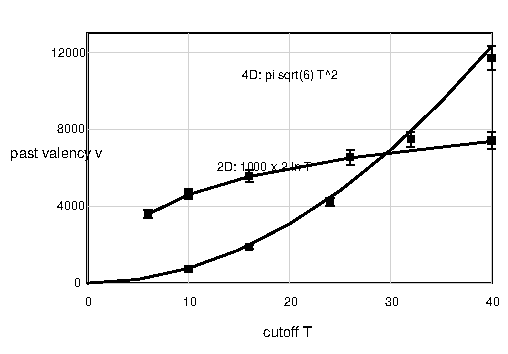
\includegraphics[width=0.62\textwidth]{figs/F1_valency_flat_laws.pdf}
\caption{Past valency vs.\ cutoff: 2D logarithmic law and 4D area law. The
4D area-law curve is parameter-free ($\kappa_{4}=\pi\sqrt{6}$); in 2D the
slope 2 is derived and the $O(1)$ offset is fitted.}
\end{figure}

\section{Results II: matter-dominated FRW}
\label{sec:frw}

Expansion should suppress valency: comoving neighbours recede, and the
effective density in conformal coordinates is diluted by powers of the scale
factor. The question is whether the area law survives and with what amplitude.

\paragraph{Transient.} At small conformal extent $\eta$ the valency is
dominated by a boundary transient. The ensemble is fit well by
$v(\eta) = A\,\eta^{2}(1 - B/\eta)$; against a free-power alternative the
transient model wins at $\Delta\mathrm{AIC} = +40.7$. We flag a warning for
future work: a naive short-range power-law fit to the same data returns an
exponent of $2.70 \pm 0.07$---the transient contaminates the exponent long
before it is visually obvious. An early soft-estimator run produced $2.95$ for
the same quantity; both numbers are artifacts, of the fit range and of the
$e^{-\rho V}$ approximation respectively, and both are superseded by the
exact-blocker, transient-subtracted analysis.

\paragraph{Asymptote.} Once the transient is subtracted, the area law
reappears with a suppressed amplitude:
\begin{equation}
  v(\eta) \;\to\; \kappa_{4}\,\mathfrak{F}\,\sqrt{\rho_{c}}\,\eta^{2},
\end{equation}
where $\rho_{c}$ is the comoving density and the blocking factor is a definite
integral over the interval's volume-weighted expansion history. For matter
domination ($a \propto \eta^{2}$) with the diamond weight
$w(s) = 32\min(s,1-s)^{3}$,
\begin{equation}
  \mathfrak{F} \;=\; 30\int_{0}^{1}
  \frac{x(1-x)^{8}}{\sqrt{\langle a^{4}\rangle}}\,dx \;=\; 0.4991,
\end{equation}
with $\langle a^{4}\rangle$ the diamond-weighted average of $a^{4}$ along the
interval. The measured amplitude ratio is $0.4990$---agreement to four
figures, again with nothing fitted.

The physical reading is modest and exact: expansion does not change the
\emph{form} of the valency law; it renormalizes the amplitude by a computable
average of the expansion history over the causal interval. All the geometry
enters through $\langle a^{4}\rangle$.

\begin{figure}[htb]
\centering
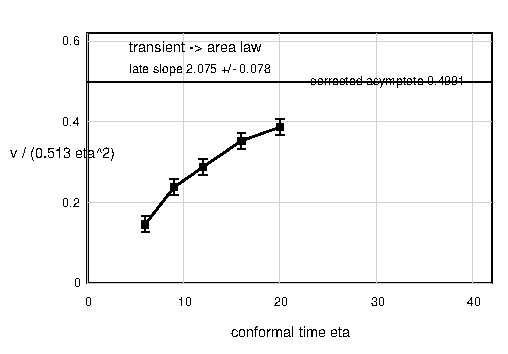
\includegraphics[width=0.62\textwidth]{figs/F2_frw_transient_amplitude.pdf}
\caption{Matter-dominated FRW: amplitude ratios converging to the derived
blocking factor $\mathfrak{F}=0.4991$, with the $1/\eta$ transient fit.}
\end{figure}

\section{Results III: the link fraction}
\label{sec:epsilon}

Valency divided by the size of the causal past gives a dimensionless,
cutoff-dependent scarcity measure:
\begin{equation}
  \varepsilon(\rho, R) \;=\; \frac{N_{\mathrm{links}}}{N_{\mathrm{past}}}
  \;\simeq\; \frac{3\sqrt{6}}{\sqrt{\rho}\,R^{2}}
  \qquad (\text{asymptotically}),
\end{equation}
which follows from the area law and the $R^{4}$ volume growth of the past
interval; at finite size the measured value tracks this asymptote with
${\approx}10\%$ boundary corrections at our scales. The headline reproduction is bit-exact
from a clean checkout (declared seeds).

$\varepsilon$ is also a cheap \textbf{manifoldlikeness discriminator}. At the
reference scale ($\sqrt{\rho}R^{2}$ such that
$\varepsilon_{\mathrm{manifold}} \approx 0.21$), a transitively-closed random
order---a Kleitman--Rothschild-like non-geometric poset---yields
$\varepsilon \approx 0.017$: an order of magnitude below the sprinkled value,
because transitive closure of random relations manufactures long chains that
de-link almost every pair. One number, computable in $O(N^{2})$ from the
causal matrix, separates the two classes without interval-abundance machinery.

We note without further claim that $\varepsilon(T) \propto T^{-2}$ places this
quantity in the well-known family of inverse-square horizon scalings
(Cohen--Kaplan--Nelson bounds, everpresent-$\Lambda$ heuristics): any $T^{-2}$
law evaluated at the Hubble scale returns a number of order $10^{-122}$. This
is a reformulation within that family, not a discovery, and we make no
cosmological use of it here.

\begin{figure}[htb]
\centering
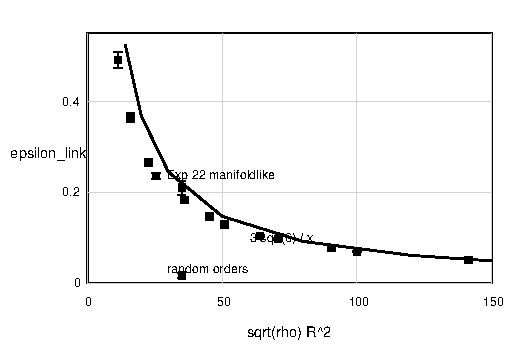
\includegraphics[width=0.62\textwidth]{figs/F3_link_fraction_manifoldness.pdf}
\caption{Link fraction $\varepsilon$ vs.\ $\sqrt{\rho}R^{2}$ collapsing to
the predicted $3\sqrt{6}/(\sqrt{\rho}R^{2})$ curve; manifoldlike sprinklings
vs.\ transitively-closed random orders separate by an order of magnitude.}
\end{figure}

\section{Outlook}
\label{sec:outlook}

The counting objects of this paper---chains (timelike depth), antichains
(spacelike width), and links---suggest one forward-looking consistency
statement. For a weakly disformal rescaling of a metric
\cite{Bekenstein1993}, $ds^{2} = -\lambda^{-2}c^{2}dt^{2} + \lambda^{+2}dx^{2}$
to first order, a faithful sprinkling must split its volume budget as
$(\text{chains} \times \lambda^{-1}) \times (\text{antichains} \times
\lambda^{+3}) = \sqrt{-g} = \lambda^{+2}$, whereas the conformal counterpart
(clocks and rulers scaled together) gives $\sqrt{-g} = \lambda^{-4}$ with both
sectors contracted---an opposite-sign, countable prediction. This is a
bookkeeping identity, not a result of this paper; its value is that it is
directly testable, which motivates the first item below. Three follow-ups are
defined and, where marked, pre-registered.

\begin{enumerate}
\item \textbf{Estimator test in a disformal metric (pre-registered):} a
  uniform sprinkling \emph{into} the weakly disformal geometry
  $ds^{2} = -\mathcal{R}^{-2}dt^{2} + \mathcal{R}^{2}d\vec{x}^{\,2}$, where
  the partition identity above predicts $(-1,+3)$ analytically. The test
  checks that the identity survives finite size and boundaries and that
  windowed local estimators---depth in proper-radius balls, width by the
  causal-overlap method of Bogu\~n\'a \& Krioukov \cite{BogunaKrioukov2024}
  rather than raw adjacency, which is asymptotically silent---can \emph{see}
  the signature. Chain lengths in inhomogeneous (Schwarzschild) sprinklings
  have been studied \cite{Eichhorn2026}; the disformal partition test appears
  to be new. Whether any \emph{growth dynamics} produces this split is a
  separate, open question deferred to future work.
\item \textbf{Link fraction in FRW:} whether $\varepsilon(T)$ and its $T^{-2}$
  scaling survive expansion with the same $\mathfrak{F}$-type renormalization
  as the valency law.
\item \textbf{Estimator hygiene:} the $2.70/2.95$ discrepancy of
  Section~\ref{sec:frw} is a reproducible case study in how soft link
  estimators and short-range fits bias growth exponents; we release both
  pipelines so the failure can be replayed.
\end{enumerate}

All code, pre-registration documents, per-experiment results files, and the
exact seeds behind every number in this paper are public in the project
repository. Negative results and superseded estimates are retained, not
deleted.

\section*{Acknowledgments}

This work grew out of a broader phenomenological programme by the author,
documented in the same public repository. The author acknowledges
computational and analytical assistance from AI systems (Anthropic Claude,
OpenAI Codex, and local models); all results are independently reproducible
from the public repository with the declared seeds.

\begin{thebibliography}{99}
\bibitem{BLMS1987} L.~Bombelli, J.~Lee, D.~Meyer, R.~D.~Sorkin,
  \emph{Space-time as a causal set}, Phys.\ Rev.\ Lett.\ \textbf{59}, 521
  (1987).
\bibitem{RideoutSorkin2000} D.~P.~Rideout, R.~D.~Sorkin, \emph{Classical
  sequential growth dynamics for causal sets}, Phys.\ Rev.\ D \textbf{61},
  024002 (2000).
\bibitem{Johnston2008} S.~Johnston, \emph{Particle propagators on discrete
  spacetime}, Class.\ Quantum Grav.\ \textbf{25}, 202001 (2008),
  arXiv:0806.3083.
\bibitem{RideoutWallden2009} D.~Rideout, P.~Wallden, \emph{Spacelike distance
  from discrete causal order}, arXiv:0810.1768.
\bibitem{BenincasaDowker2010} D.~M.~T.~Benincasa, F.~Dowker, \emph{The scalar
  curvature of a causal set}, Phys.\ Rev.\ Lett.\ \textbf{104}, 181301 (2010),
  arXiv:1001.2725.
\bibitem{GlaserSurya2013} L.~Glaser, S.~Surya, \emph{Towards a definition of
  locality in a manifoldlike causal set}, Phys.\ Rev.\ D \textbf{88}, 124026
  (2013), arXiv:1309.3403.
\bibitem{Surya2019} S.~Surya, \emph{The causal set approach to quantum
  gravity}, Living Rev.\ Relativ.\ \textbf{22}, 5 (2019), arXiv:1903.11544.
\bibitem{BB1991} B.~Bollob\'as, G.~Brightwell, \emph{Box-spaces and random
  partial orders}, Trans.\ Amer.\ Math.\ Soc.\ \textbf{324} (1), 59--72
  (1991); \emph{The height of a random partial order: concentration of
  measure}, Ann.\ Appl.\ Probab.\ \textbf{2} (4), 1009--1018 (1992).
\bibitem{BrightwellLuczak} G.~Brightwell, M.~\L uczak, \emph{The mathematics
  of causal sets}, in \emph{Recent Trends in Combinatorics}, IMA Vol.\ Math.\
  Appl.\ 159, Springer (2016), arXiv:1510.05612.
\bibitem{Bekenstein1993} J.~D.~Bekenstein, \emph{The relation between
  physical and gravitational geometry}, Phys.\ Rev.\ D \textbf{48}, 3641
  (1993), arXiv:gr-qc/9211017.
\bibitem{Eichhorn2026} A.~Eichhorn, T.~Gamito, D.~Stokes, \emph{Towards
  black-hole horizons and geodesic focusing in causal sets},
  arXiv:2605.06813.
\bibitem{Glaser2023} L.~Glaser, arXiv:2306.09904.
\bibitem{BogunaKrioukov2024} M.~Bogu\~n\'a, D.~Krioukov, \emph{Spatial
  distances in causal sets}, Phys.\ Rev.\ D \textbf{110}, 024008 (2024),
  arXiv:2401.17376.
\bibitem{Johnston2022} S.~Johnston, arXiv:2111.09331.
\bibitem{Johnston2025} S.~Johnston, arXiv:2502.09701.
\end{thebibliography}

\end{document}
